%!TEX root = main.tex

\section{Understanding Web Search Performance}
\label{sec:web_search}

In this section, we examine the TCP performance of web search flows. We start by providing high-level statistics on key performance indicators in Table~\ref{tab:web_stats}. For flow completion time, flow size and RTT, we report the median along with the $5th$ and $95th$ percentile values in parenthesis. Flow size measures the number of web search result packets as show in Figure~\ref{fig:web_finish_time_example}. We observe that 3G flows are larger than WiFi's, which can be explained by the difference in search behavior across these access technologies \cite{Song:2013:EEU:2488388.2488493}. Most of the flows contain no more than 100 packets, hence still relatively short, implying that any TCP performance degradation (\eg high packet loss) could exert a large influence on user perceived latency (\ie flow completion time)~\cite{flach2013reducing}. Flow size does not affect performance though, with little correlation between these two variables (the Kendall correlation coefficient is 0.018. Overall, 3G flows exhibit smaller RTT, lower packet loss rate and also are less likely to suffer from timeout retransmissions.

As a TCP sender in web search, the server is able to measure multiple TCP performance factors and behavior, enabling us to perform a detailed analysis of the TCP performance and its impact on the flow completion time. In the sequel, we analyze the TCP performance across the 3 main TCP phases, and in particular detail delve into timeout retransmissions.

\subsection{TCP Phase Analysis}

\begin{figure}[th]
\centering
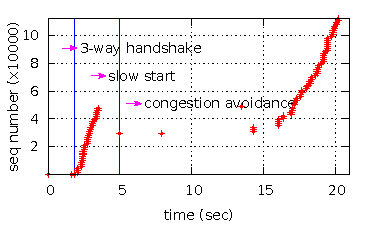
\includegraphics[width=0.8\linewidth]{web_three_stages}
\caption{The three phases in web search flows.}
\label{fig:web_three_stages}
\minsqueeze
\end{figure}

A TCP flow comprises 3 phases: \emph{3-way handshake}, \emph{slow start}, and \emph{congestion avoidance}, which is illustrated in Figure~\ref{fig:web_three_stages} using a web search flow from our dataset, where the $y$-axis shows the TCP sequence number. The TCP 3-way handshake (3WHS) phase ideally completes within 1 RTT (\ie without packet loss, delay and reordering). The server then enters the slow start phase, during which the server does not encounter any packet loss or reordering event, and thus increases the congestion window by 1 segment for each received ACK. The server enters congestion avoidance phase once it detects a packet loss\footnote{The packet can actually be delayed or lost.} and retransmits the packet. In this phase, the server decreases the congestion window when detecting packet loss through 3 dupacks~\cite{rfc6675} and sets the congestion window to 1 segment when detecting packet loss through RTO. Note that the congestion avoidance phase here starts when the server detects congestion and retransmits packet, and ends when the flow terminates, which is slightly different from the TCP congestion avoidance phase in TCP stack~\cite{jacobson1988congestion}.

\subsubsection{3-way Handshake}

\begin{figure}[th]
\centering
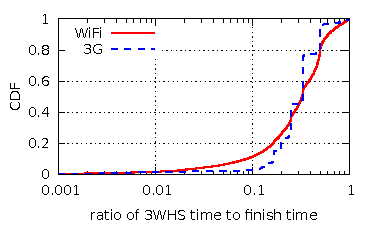
\includegraphics[width=0.8\linewidth]{web_handshake_time_ratio}
\caption{The ratio of time in 3-way handshake to completion time in each flow.}
\label{fig:web_handshake_ratio}
\minsqueeze
\end{figure}

We first examine how much of the time flows spend in the 3WSH phase (Figure~\ref{fig:web_handshake_ratio}). Figure~\ref{fig:web_handshake_ratio} shows the CDF of the ratio between the time in 3WSH and the flow completion time, using a log scale for the $x$-axis. 3G and WiFi flows spend a comparable ratio of their time in this phase. We observe that the time spent during connection establishment can take as much as half of the flow completion time for 30\% flows. About 8\% of the WiFi flows and 3\% of 3G flows spend as much as 70\% of their time during this phase. The small flow size is one of the reasons for this. Indeed, the maximum flow size is 100 packets, as shown in Table~\ref{tab:web_stats}, implying that the data has very few RTTs to be transmitted, if no congestion event happens. Obviously, such a short period of transmission time leads to a relatively large portion of time for connection establishment.

%From the figure, flows in cellular network have similar ratio of time in 3-way handshake to that in WiFi network (with median value 0.3). If the 3WSH could be removed from flow completion time, the user-perceived web search latency would be reduced by 30\% in more than half of the flows. Moreover, there are 8\% of flows in WiFi network consuming 70\% of their time in 3WSH.

%The unexpectedly high ratio of 3WSH could be introduced by two reasons. First, most of web search flows contains packets ranging from 1 to 100, these data could transmitted in 1 to 4 RTT's if there is no congestion event. Thus 3WHS, without transmitting any data, occupies a large fraction of time in short flows. Second, there are a non-negligible fraction of flows experiencing SYN retransmission during 3WHS phase. 

Another important reason that explains the unexpectedly long time spent in the 3WSH phase (\ie $>70\%$ of flow completion time) are timeout retransmissions. As data packets cannot be transmitted before a TCP connection is established, a loss of SYN will lead to a timeout retransmission, which takes 1 second (\ie the initial RTO) to retransmit the SYN. We find that 4.4\% of WiFi search flows and 0.5\% of 3G flows experience at least one SYN timeout retransmission. A timeout retransmission for a SYN also sets the congestion window to 1, further hurting the data transmission performance by negating the benefits of the value of the initial congestion window. 
% We envision a possible way to mitigate the costly 3WSH in such short flows where clients maintain long-term TCP connections to the web search servers.
% Steve: so what's the solution? I'd say force the initial congestion window size to a default, e.g., 10, and not to go to 0.

\subsubsection{Slow Start Phase}

\begin{figure}[th]
\centering
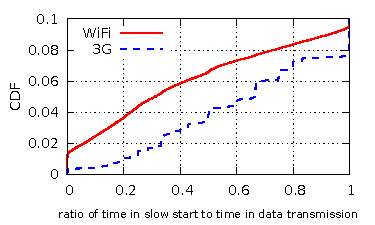
\includegraphics[width=0.8\linewidth]{web_slowstart_time_ratio}
\caption{Ratio of time spent in slow start to the time in data transmission (slow start and congestion avoidance).}
\label{fig:web_ss_time_ratio}
\minsqueeze
\end{figure}

The slow start and the congestion avoidance phases constitute the data transmission period of a flow. Figure~\ref{fig:web_ss_time_ratio} shows the ratio of time in slow start phase to the time spent in data transmission (\ie the sum of time in slow start and congestion avoidance). Note that the $y$-axis is capped at 0.1. We observe that 1.5\% of the WiFi flows are unable to transmit any data in the slow start phase, because their first packet is dropped.

\begin{table}[th]
\caption{Comparison of flow completion time (ms) for flows finishing during the slow start phase and those not.}
\label{tab:web_finish_time_3rd_phase}
\centering
\renewcommand{\arraystretch}{1.0}
\begin{tabular}{l|c|c|c}
\hline
& 5 \%ile & median & 95 \%ile \\
\hline
WiFi finished & 30 & 170 & 2,810 \\
WiFi unfinished & 80 & 770 & 21,240 \\
\hline
3G finished & 10 & 120 & 810 \\
3G unfinished & 10 & 160 & 2,420 \\
\hline
\end{tabular}
\minsqueeze
\end{table}

More importantly, regardless of the access technology, more than 90\% of the flows finish during the slow start phase. In other words, about 10\% of the flows have to experience the congestion avoidance phase. Intuitively, the more time spent in the slow start phase, the shorter the time to complete the data transmission. To verify this, we compare in Table~\ref{tab:web_finish_time_3rd_phase} the flow completion time of the flows that finish in the slow start phase and those who do not. Overall, increasing the likelihood of finishing web search results transfer during slow start can greatly improve the user perceived latency. For example, the median flow completion time would be improved by 4 times if a flow finishes in the slow start phase instead of entering the congestion avoidance phase. The 95th percentile flow completion time can be improved by one order of magnitude. We also observe that WiFi flows are more impacted if they do not finish during slow start.

\begin{table}[th]
\caption{Correlation between RTT and flow completion time.}
\label{tab:web_rtt_finish_time_correlation}
\centering
\renewcommand{\arraystretch}{1.0}
\begin{tabular}{c|C{2.6cm}|C{2.5cm}}
   \hline
   & w/o cong. avoid. & w/ cong. avoid. \\
   \hline
   WiFi & 0.55 & 0.13 \\
   3G & 0.59 & 0.52 \\
   \hline
\end{tabular}
\minsqueeze
\end{table}

During the slow start phase, the congestion window is doubled after each RTT. Suppose there is no packet loss, for a flow containing $k$ data packets, sender requires $\lceil{\log_2 (k/10+1)}\rceil$ RTTs to transmit all the packets. Thus it takes about 4 RTTs to transmit 100 data packets if there is no packet loss. According to the formula above, the RTT is expected to have a high impact on the flow completion time. To confirm this, we examine in Table~\ref{tab:web_rtt_finish_time_correlation} the Kendall correlation between RTT and flow completion time, for flows that finish in the slow start phase (\ie without entering congestion avoidance). For comparison, we also report the correlation for flows that experience congestion avoidance. We observe, regardless of the access technology, a mild correlation for flows that finish in the slow start phase, confirming the expected impact of RTT on the flow completion time for these flows. The correlation for flows that experience congestion avoidance however is dependent on the access technology, which can be explained by the fact that other factors, such as packet loss, can have a significant impact during the congestion avoidance phase. As we have seen in Table~\ref{tab:web_stats}, WiFi flows experience a higher packet loss rate and thus are more likely to be impacted by packet loss than RTT. In addition, as we will see in the following analysis, WiFi flows that experience the congestion avoidance are more likely to recover packet losses through expensive timeout retransmissions.

\subsubsection{Congestion Avoidance Phase}

\begin{figure}[th]
\centering
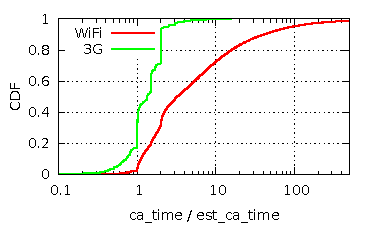
\includegraphics[width=0.8\linewidth]{web_ca_prac_over_est}
\caption{CDF of the extra time introduced by the congestion avoidance phase.}
\label{fig:web_ca_round}
\minsqueeze
\end{figure}

We first examine how much extra time the congestion avoidance phase introduces for individual flows. Let $\#(ca\_pkts)$ be the number of packets transmitted in this phase for a flow. As a TCP sender, the server sends $cwnd$ packets in one RTT, where $cwnd$ is the size of the congestion window at the time of entering the congestion avoidance phase. Thus, if the flow had not experienced the congestion avoidance phase, the server would have sent $\#(ca\_pkts)$ packets over a time duration of $T_e =  \left \lceil{ \log_2 (\frac{\#(ca\_pkts)}{cwnd}}+1) \right \rceil \times RTT$. Now, we observe that the flow actually spent $T_r$ of time for transmitting these packets. Then we compute the ratio of  $T_r$ to $T_e$ and use this ratio to quantify the extra time introduced by this phase. Unfortunately, we do not see $cwnd$ from the traces, and instead use the number of in-flight packets at the time of entering the phase to approximate this value~\cite{rfc56812009tcp}. 
 
Figure~\ref{fig:web_ca_round} reports the distribution of this ratio. We observe a surprisingly high ratio for WiFi flows. The median ratio is as high as 3.2 and 20\% of the WiFi flows have a ratio higher than 11, meaning that 10 times more time is necessary to complete the flow for these 20\% of flows. 3G flows on the other hand have a ratio no larger than 2, for 95\% of the flows. The difference between 3G and WiFi flows in the packet loss rate (3\% in WiFi versus 0.9\% in 3G) and the difference in the impact of packet loss largely contribute to the observed difference between WiFi and 3G flows.

\begin{table}[th]
\caption{Flow completion time (in ms, represented as median (5th percentile, 95th percentile)) under different numbers of lost packets.}
\label{tab:web_loss_finish_time}
\centering
\renewcommand{\arraystretch}{1.0}
\begin{tabular}{c|c|c}
\hline
\#(lost pkts) & WiFi & 3G\\
\hline
0 & 180 (30, 3,200) & 120 (10, 570) \\
%
1 & 480 (50, 12,070) & 220 (40, 570) \\
%
2 & 540 (80, 14,460) & 230 (40, 590) \\
%
$\ge$3 & 2,820 (140, 34,890) & 270 (50, 930) \\
\hline
\end{tabular}
\minsqueeze
\end{table}

We then examine the impact of packet loss on flow completion time in Table~\ref{tab:web_loss_finish_time}. Flows are grouped based on how many packets were lost in individual flows. The median flow completion time, along with the $5th$ and $95th$ percentiles are reported for each group. For comparison, we also report the statistics for flows without any packet loss, \ie these flows finish the data transmission in the slow start phase. For 3G flows, a packet loss nearly doubles the flow completion time compared to the flows with no packet loss. A higher number of packet losses does not increase the flow completion time significantly in 3G. The situation for WiFi is different, with every additional packet loss leading to an even more pronounced increase in the flow completion time: the median flow completion time increases from 180 ms for flows with no packet loss to 480 ms for flows with 1 lost packets, and grows up to 2.8 second for flows with more than 3 lost packets. 

The huge difference in the impact of packet loss on flow completion time for WiFi and 3G flows is related to how the packet loss is recovered. A packet loss can be recovered by fast retransmit, early retransmit~\cite{rfc5827}, or timeout retransmission by the server\footnote{TLP \cite{flach2013reducing} is not enabled at the server.}. Among these possible recovery methods, the most expensive one is timeout retransmission, which is indeed the factor that explains the difference between WiFi and 3G flows in Table~\ref{tab:web_loss_finish_time}, as the following analysis reveals.

\subsection{Timeout Retransmission Analysis}

\begin{figure}[th]
\centering
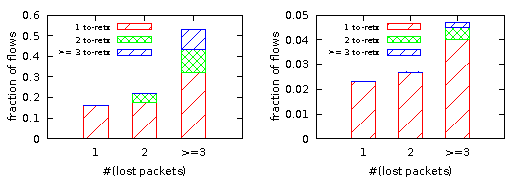
\includegraphics[width=\linewidth]{web_loss_rto_ratio}
\caption{Fraction of flows with timeout retransmission under different number of lost packets.}
\label{fig:web_loss_rto_ratio}
\minsqueeze
\end{figure}

A retransmission is identified as a timeout retransmission if this retransmission happens at least RTO after the transmission of the previous packet. The RTO here is computed as~\cite{rfc62982011computing} $$RTO=\text{SRTT} + max(200ms, 4 \text{ RTTVAR}) \enspace ,$$ where SRTT is the smoothed value of all measured RTTs, and RTTVAR is the variation of RTTs. We examine the fraction of flows that experience timeout retransmission(s) given the number of lost packets in Figure~\ref{fig:web_loss_rto_ratio}. Note that the two sub-figures have different $y$-axis limits. We can see that WiFi flows are more likely to suffer from timeout retransmissions than 3G flows. Given the same number of lost packets, the fraction of WiFi flows suffering from timeout retransmissions is about one order of magnitude higher than for 3G flows. 20\% of WiFi flows suffering from more than 3 packets lost experience more than 2 timeout retransmissions, potentially leading to a serious performance degradation. This percentage however is only 1\% for 3G flows.

A natural question at this point is \textit{``why are timeout retransmissions more likely to happen for WiFi than 3G flows?''}. To answer this question, we need to nail down the reasons behind each timeout retransmission. Essentially, there are two scenarios in which a TCP sender has to recourse to timeout retransmission for loss recovery. The first scenario is that the retransmitted packet issued to recover the loss, for example by fast retransmit, is dropped by network. In this case, the sender has to wait for a duration equal to RTO to recover the packet loss (referred to as \emph{double retransmission}). 

The second scenario is that the sender cannot collect enough duplicate acknowledgments (\emph{dupacks}) to trigger fast retransmit. The limited number of dupacks could be caused by various reasons: (1) the packet loss happened in the last 3 packets of a flow, referred to as \emph{tail retransmission}~\cite{flach2013reducing}; (2) the congestion window is too small (\eg 1 segment), referred to as \emph{small cwnd retransmission}; or (3) the lost packet is followed subsequently by other packets with higher sequence numbers and the ACKs of subsequent packets are delayed for a long time (longer than a RTO), referred to as \emph{packet delay retransmission}. The last case might be caused by large network jitter or middleboxes blocking the disordered packets~\cite{Wang:2011:USM:2018436.2018479}.

\begin{algorithm}
	\caption{Process of determining the type of timeout retransmission.}
	\label{alg:rto}
	\begin{algorithmic}[1]
		\Procedure{ParseRTO}{$timeout\ retx$}
			\If {packet has been retransmitted}
				\State \textbf{return} $double\_retransmission$
			\ElsIf {position to tail $\le$ 3}
				\State \textbf{return} $tail\_retransmission$
			\ElsIf {\#(in-flight packets) == 1}
				\State \textbf{return} $small\_cwnd\_retransmission$
			\ElsIf {only 1 in-flight packet is dropped \textbf{and}
				\Statex \indent\indent\indent\indent no dupack is received}
				\State \textbf{return} $packet\_delay\_retransmission$
			\Else
				\State \textbf{return} $other$
			\EndIf
		\EndProcedure
	\end{algorithmic}
\end{algorithm}

We use the methodology shown in Algorithm~\ref{alg:rto} to determine the type of timeout retransmission. Those that cannot be classified into any of the above type (\eg when all packets in the window are dropped) are labeled as ``other''. Table~\ref{tab:rto_type} reports the fraction of timeout retransmissions classified into each type.

\begin{table}[th]
\caption{Types of timeout retransmissions.}
\label{tab:rto_type}
\centering
\renewcommand{\arraystretch}{1.0}
\begin{tabular}{c|C{1.1cm}|C{1.1cm}}
	\hline
	{timeout retx type} & WiFi & 3G \\
	\hline
	tail retx & 38.3\% & 69.6\% \\
	double retx & 33.8\% & 13.5\% \\
	packet delay retx & 27.4\% & 16.1\% \\
	small cwnd retx & 0.3\% & 0.6\% \\
	others & 0.2\% & 0.2\%\\
	\hline
\end{tabular}
\minsqueeze
\end{table}

Tail retransmission contributes the majority (\ie 70\%) of timeout retransmissions for 3G flows. Indeed, if the packet loss happens in the tail of a flow, it has to be recovered through timeout retransmission. Given the small size of web search flows, a tail packet loss can lead to a notable increase of the flow completion time~\cite{flach2013reducing}. However, in WiFi flows, only 38\% of the timeout retransmissions are classified as tail retransmissions, because double retransmission and packet delay retransmission are much more likely than in 3G flows. The higher probability of double retransmission in WiFi flows might come from the higher packet loss rate, in which case the retransmitted packet itself is dropped. On the other hand, the higher probability of packet delay retransmission implies a possibility that in WiFi network that we examined, middleboxes might buffer the disordered packets. We leave the examination of the impact of middleboxes as future work.

The results in Table~\ref{tab:rto_type} explain why timeout retransmissions are more likely to happen in WiFi flows: besides tail retransmissions, the loss of the retransmitted packet and the delayed ACKs also increase the likelihood of timeout retransmissions for WiFi flows, but they contribute much less in 3G flows. Our observations also imply that besides mitigation methods for tail retransmission, \eg TLP~\cite{flach2013reducing}, there is a need for methods to mitigate double retransmissions and packet delay retransmissions, especially in WiFi networks.

\subsection{Summary of web search analysis}

The key observations on web search flows are summarized below:

\begin{itemize}

\item More than 50\% of flows spend at least 30\% of their total time in connection establishment. Moreover, 4.4\% of WiFi flows have to retransmit the SYN packet, making the time for establishing connections longer than 1 second.
	
\item Independent of access type, 90\% of the flows experience no packet loss and thus finish in the slow start phase. For these flows,  RTT plays an important role in the flow completion time. %However, in the flows with packet loss, the time spent on loss recovery dominates the flow completion time.
	
\item For those flows with packet loss, the time taken for loss recovery makes the flow completion time at least 2-3 times larger. Compared with 3G flows, WiFi flows are more sensitive to packet loss, partially because WiFi flows are more likely to use timeout retransmission for packet recovery. 
	
\item Most timeout retransmissions in 3G network are induced by packet losses in the flow tail. However, tail retransmission, double retransmission and packet delay retransmission contribute very close (38.3\%, 33.8\% and 27.4\% respectively) in WiFi flows. 
	
\end{itemize}